%!TEX program = xelatex

\documentclass{beamer}
% \documentclass[aspectratio=169]{beamer}
\usepackage{SPL-beamer}
\usepackage{multimedia}
\usepackage{marvosym}

\mode<presentation>
{
    \usetheme{WarsawLite}
}

\setbeamertemplate{footline}{}

\AtBeginSection[]{
  \begin{frame}
  \vfill
  \centering
  \begin{beamercolorbox}[sep=8pt,center,shadow=true,rounded=true]{title}
    \usebeamerfont{title}\insertsectionhead\par%
  \end{beamercolorbox}
  \vfill
  \end{frame}
}


\title{Electrical and Information Engineering}
\author[]{Alex Maraschin and Stephen Levitt\\ \vspace{3mm}
\href{mailto:469699@students.wits.ac.za}{469699@{\small\MVAt}students.wits.ac.za}\\
\href{mailto:stephen.levitt@wits.ac.za}{stephen.levitt{\small\MVAt}wits.ac.za}}

\begin{document}

\titleslide

\begin{frame}
    \frametitle{Outline}
    \tableofcontents[hideallsubsections]
\end{frame}

% \begin{itemize}
%   \item Ask about parents or family being engineers
%   \item This leads to the definition of what is an engineer
% \end{itemize}

\section{What is an engineer?}


\begin{frame}
\begin{unsignedquote}
 \textit{Engineer}: a person who has scientific training and who designs and builds complicated products, machines, systems, or structures.
\end{unsignedquote}

\vspace{5mm}

\begin{unsignedquote}
 \textit{Engineer}:  a person who uses scientific knowledge to \alert{solve practical problems}.
\end{unsignedquote}
\end{frame}

\section{What do engineers do?}
\begin{frame}
\frametitle{What kinds of problems do engineers solve?}
  \begin{enumerate}
    \item How can we ensure that everyone gets energy for lighting, cooking, and hot water?
    \item How do we reduce the number of road accidents?
    \item How do we make it easy to find relevant information on the internet?  
  \end{enumerate}

  And many others \ldots

\end{frame}

\subsection{Energy for Everyone}
\begin{frame}[plain,c]
\begin{center}
\Huge Energy for Everyone
\end{center}
\end{frame}


\begin{frame}
  \frametitle{Electricity Production in Africa}
  \begin{figure}
  \centering
  \includegraphics[width=\linewidth,height=\textheight,keepaspectratio]{energy/elec-africa}
  \end{figure}
\end{frame}

% South Africa and Egypt

\begin{frame}
\frametitle{Africa at Night}
  \begin{figure}
  \centering
  \includegraphics[width=\linewidth,height=\textheight,keepaspectratio]{energy/earth-at-night}
  \end{figure}  
\end{frame}

\begin{frame}
  \frametitle{Coal-Fired Power Station - Arnot}
  \begin{figure}
  \centering
  \includegraphics[width=\linewidth,height=\textheight,keepaspectratio]{energy/arnot}
  \end{figure}
\end{frame}

% Problem of running out of fossil fuels, problem of pollution, problem of distribution

\begin{frame}
  \frametitle{Energy for Everyone - Solutions}
{\Large
\begin{itemize}
  \item Produce more
  \item Consume less
\end{itemize}}
\end{frame}


\begin{frame}
  \frametitle{Shack with Solar Power}
  \begin{figure}
  \centering
  \includegraphics[width=\linewidth,height=\textheight,keepaspectratio]{energy/shack-solar}
  \end{figure}
\end{frame}

\begin{frame}
  \frametitle{Windfarm in Darling (Western Cape)}
  \begin{figure}
  \centering
  \includegraphics[width=\linewidth,height=\textheight,keepaspectratio]{energy/wind-energy-small}
  \end{figure}
\end{frame}

\begin{frame}
  \frametitle{Geyser Blankets}
  \begin{figure}
  \centering
  \includegraphics[width=\linewidth,height=\textheight,keepaspectratio]{energy/geyser}
  \end{figure}
\end{frame}

\begin{frame}
  \frametitle{LED Lighting}
  \begin{figure}
  \centering
  \includegraphics[width=\linewidth,height=\textheight,keepaspectratio]{energy/genmin}
  \end{figure}
\end{frame}

\subsection{Self-Driving Cars}
\subsection{Energy for Everyone}
\begin{frame}[plain,c]
\begin{center}
\Huge Reducing Road Accidents
\end{center}
\end{frame}


\begin{frame}
  \frametitle{Google's Self-Driving Car}
  \begin{figure}
  \centering
  \includegraphics[width=\linewidth,height=\textheight,keepaspectratio]{self-driving-car/car-front-2}
  \end{figure}
\end{frame}

% 

\begin{frame}
  \frametitle{How it Works}
  \begin{figure}
  \centering
  \includegraphics[width=\linewidth,height=\textheight,keepaspectratio]{self-driving-car/how-it-works}
  \end{figure}
\end{frame}

\begin{frame}
  \frametitle{Global Positioning System or GPS}
  \begin{figure}
  \centering
  \includegraphics[width=\linewidth,height=\textheight,keepaspectratio]{self-driving-car/gps}
  \end{figure}
\end{frame}


\subsection{Google Search}
\begin{frame}[plain,c]
\begin{center}
\Huge Finding Information Online
\end{center}
\end{frame}

%  40 million searches per second, about a million machines, indexing a trillion pages

\begin{frame}
  \frametitle{Google Search}
  \begin{figure}
  \centering
  \includegraphics[width=\linewidth,height=\textheight,keepaspectratio]{google/google}
  \end{figure}
\end{frame}

\begin{frame}
  \frametitle{A Google DataCenter}
  \begin{figure}
  \centering
  \includegraphics[width=\linewidth,height=\textheight,keepaspectratio]{google/floor-small}
  \end{figure}
\end{frame}

\begin{frame}
  \frametitle{Server Racks}
  \begin{figure}
  \centering
  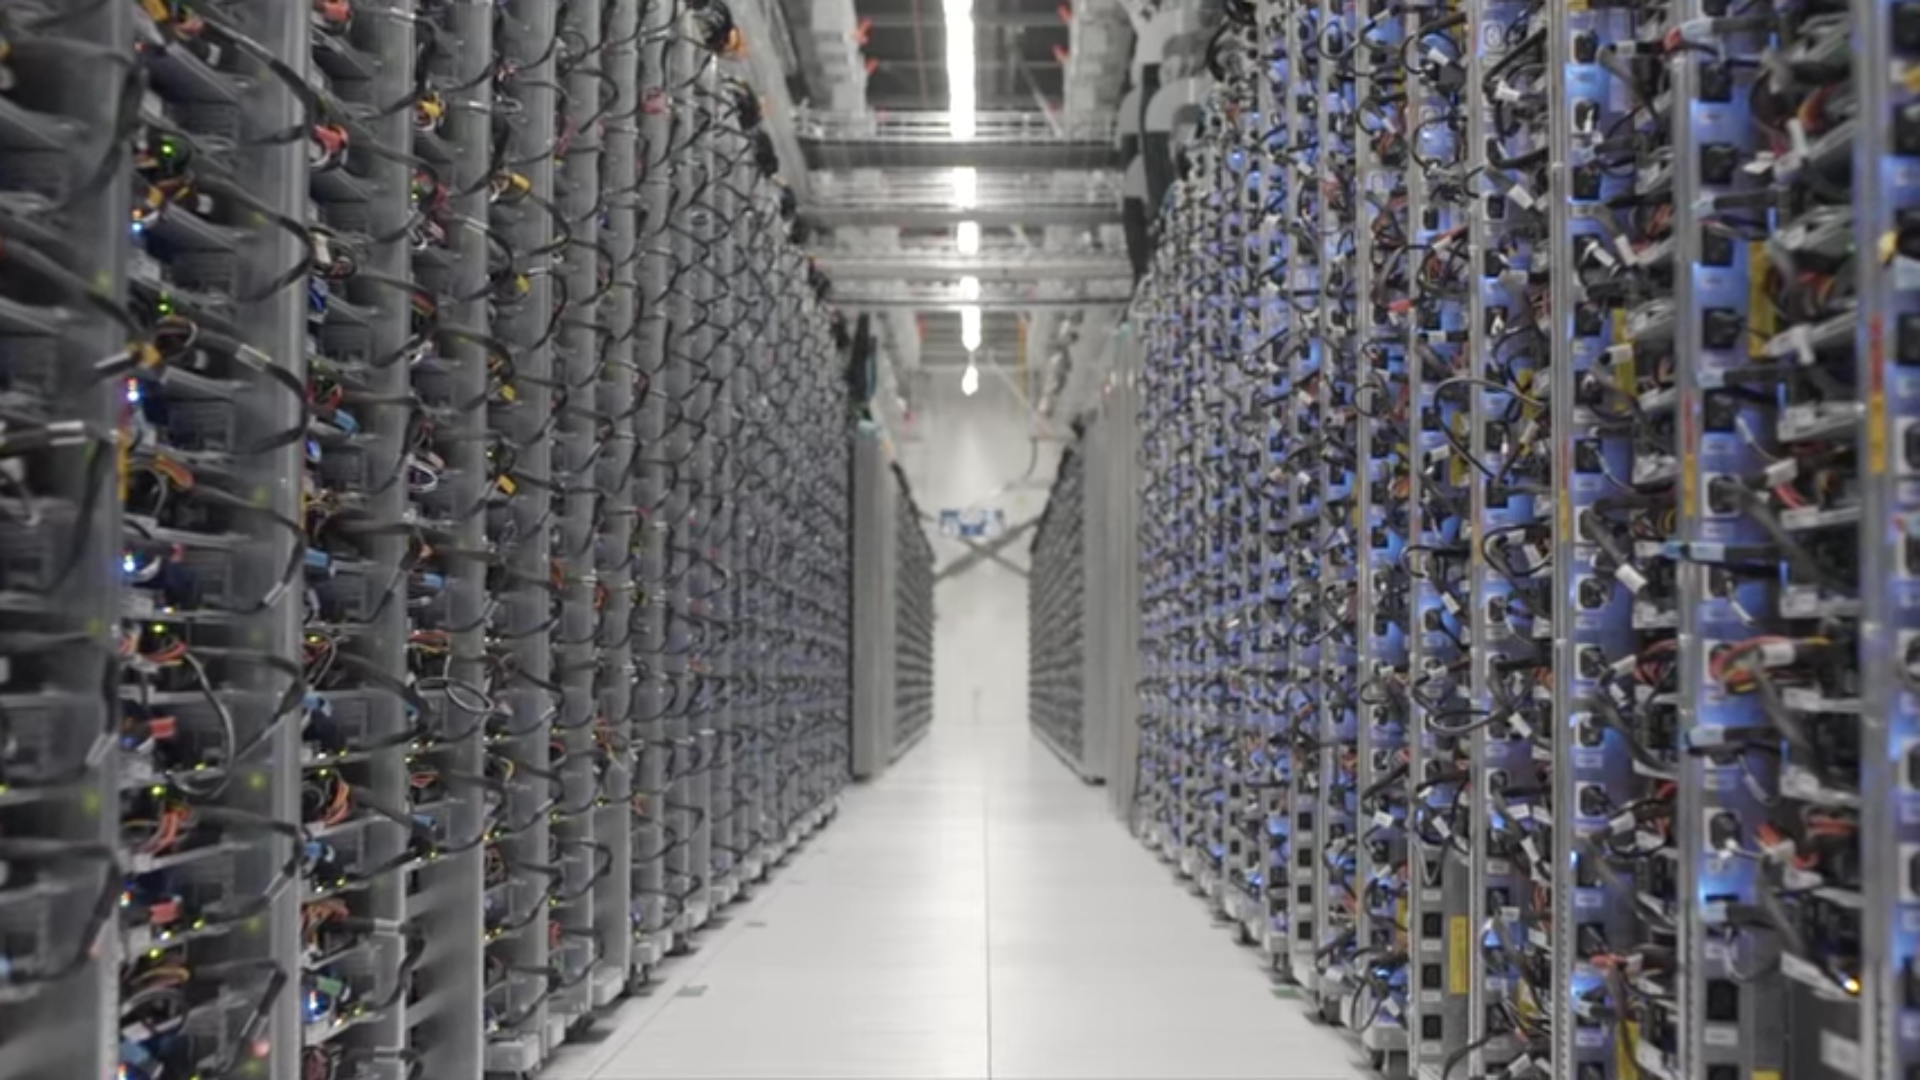
\includegraphics[width=\linewidth,height=\textheight,keepaspectratio]{google/servers}
  \end{figure}
\end{frame}

\begin{frame}
  \frametitle{The Human-Machine Interface}
  \begin{figure}
  \centering
  \includegraphics[width=\linewidth,height=\textheight,keepaspectratio]{google/human-machine}
  \end{figure}
\end{frame}

\begin{frame}
  \frametitle{Natural Language Processing}
  \begin{figure}
  \centering
  \includegraphics[width=\linewidth,height=\textheight,keepaspectratio]{google/nlp}
  \end{figure}
\end{frame}

\section{How do you become an engineer?}

\begin{frame}
\frametitle{How do you become an engineer?}
  \begin{itemize}
    \item You need to get an engineering degree from a university
    \item You need good grades, aim for 70\%, or more, in
    \begin{itemize}
      \item English
      \item Mathematics
      \item Physical Science 
    \end{itemize}
    \item APS score $\ge$ 36 
    \item Also 
    \begin{itemize}
       \item logical thinking
       \item good communication skills
       \item the ability to work well in a team
  \end{itemize}
  \end{itemize}
\end{frame}

\begin{frame}
  \frametitle{Where We Work and Study and Play at Wits}
  \begin{figure}
  \centering
  \includegraphics[width=\linewidth,height=\textheight,keepaspectratio]{wits/chamber-of-mines}
  \end{figure}
\end{frame}

\begin{frame}
  \frametitle{In the Snow!}
  \begin{figure}
  \centering
  \includegraphics[width=\linewidth,height=\textheight,keepaspectratio]{wits/cm-snow}
  \end{figure}
\end{frame}

\begin{frame}
  \frametitle{The Great Hall - Graduation}
  \begin{figure}
  \centering
  \includegraphics[width=\linewidth,height=\textheight,keepaspectratio]{wits/great-hall}
  \end{figure}
\end{frame}

\begin{frame}
\frametitle{Costs and Applying for Funding}
 First year costs about \alert{R 45 000!}\\
\vspace{3mm}
 Funding options (google: ``wits funding''):
  \begin{enumerate}
    \item Undergraduate scholarships and awards
    \begin{itemize}
    \item University entrance scholarships for APS scores $\geq$ 43
    \item Equity and sport scholarships
    \end{itemize}
    \item NSFAS loans
    \item Bursaries from Sasol, Eskom, Transnet, Telkom, Vodacom \dots
  \end{enumerate}
  \vspace{3mm}
    % \begin{itemize}
    % \item Google: ``wits funding''
  Apply early, apply for as many scholarships/bursaries as you can
      % \end{itemize}
\end{frame}

\begin{frame}[plain,c]
\begin{center}
\Huge Come and join us!
\end{center}
\end{frame}

\begin{frame}
  \frametitle{Fourth Year Lab Projects}
  Go to YouTube and search for: \\
  \vspace{5mm}
  {
    \centering
  ``wits school of electrical and information engineering''
  }
% \movie[externalviewer,width=3cm,height=2cm,poster]{}{artificial-horizon-system.mp4}
% \movie[height = 0.8\textwidth, width = 0.8\textwidth, poster, showcontrols]{}{artificial-horizon-system.mp4}
\end{frame}



\end{document}
